\appendix
\section{supplementary}


\begin{table}[h!]
	\centering
	\caption{\label{tab:approach:notation}%
		Table of notation.
	}
	\resizebox{\linewidth}{!}{%
	%    \setlength{\tabcolsep}{3pt}%
	\begin{tabular}{ c l } 
		\toprule
		\textbf{Notation} & \textbf{Meaning}  \\ 
		\midrule
		$I_t$                       & The equirectangular RGB image at time $t$. \\
		$\hat{I}_{t,i}$             & The $i$th sub-image of the cube map at time $t$.\\
		$\tilde{I}_{t,i}$           & The $i$th sub-image of the icosahedron at time $t$.\\
		$M_{\mathcal{F}}$           & The backbone optical flow method. \\
		$\mathcal{F}_t$             & Optical flow from $I_t$ to $I_{t+1}$ (equirect). \\
		$\bar{\mathcal{F}}_t$       & Optical flow from $I_t$ to $I_{t+1}$. \TODO{???} \\
		$\hat{\mathcal{F}}_{t,i}$   & Optical flow from $\hat{I}_{t,i}$ to $\hat{I}_{t+1,i}$ (cubemap). \\
		$\tilde{\mathcal{F}}_{t,i}$ & Optical flow from $\tilde{I}_{t,i}$ to $\tilde{I}_{t+1,i}$ (icosahedron). \\
		$\mathcal{R}$               & The rotation matrix estimated from optical flow. \\
		$P$                         & Pixel position $(u,v)$ in ERP image plane.   \\
		$\hat{P}$                   & Pixel location $(\theta, \phi)$ in spherical coordinate system. \\
		$T$                         & Pixel location $(x,y)$ in tangent image's gnomonic normalized coordinate system. \CR{shorten description?} \\
		$\hat{T}$                   & Pixel location $({u}',{v}')$ in tangent image's gnomonic image coordinate system. \\
		$\hat{P}'_i$                & The gnomonic projection's tangent point $\hat{P}$. \\
		\bottomrule
	\end{tabular}}%
\end{table}

\subsection{Coordinate system}



\begin{figure}[h]
	\centering
	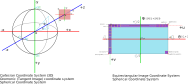
\includegraphics[width=1.0\linewidth]{images/coordinate_system.pdf}
	\caption{Coordinate system.}
	\label{fig:supp:coordinatesystem}
\end{figure}

\textbf{ERP image pixel coordinate system}

The panoramic image's $x$ and $y$ is continual, in this way it's reasonable the pixel coordinate 0 exceed the range of image pixel $([0, image\_width), [0, image\_height))$. 


\textbf{Conversion between spherical coordinate system and ERP image pixel coordinate system}


\begin{equation}\label{equ:app:sph2erp}
	\begin{split}
		\theta &= (x+0.5) \cdot\frac{2 \pi}{W_{idth}}- \pi
		\\
		x &= \frac{\theta + \pi}{\frac{2\pi}{W_{idth}}} - 0.5
		\\
		\phi&=-(y+0.5) \cdot \frac{\pi}{H_{eight}} + \frac{\pi}{2}
		\\
		y &=\frac{-\phi+\frac{\pi}{2}}{\frac{\pi}{H_{eight}}}-0.5
	\end{split}
\end{equation}


\subsection{Synthetic Dataset Generation}

The rasterization render method OpenGL used to synthesize the ground truth optical flow.
The equirectangular optical flow generation algorithm introduction in \cref{sec:app:panoof}.
Few public indoor 3D datasets are hired to render the ground truth data.

Although KITTI~\cite{Menze2018JPRS} or MPI Sintel~\cite{ButleWSB2012} pinhole image optical flow, etc.

The synthetic panoramic optical flow rendered with off-the-shelf OpenGL render pipeline and store in the ERP image.
The input are textured 3D mesh and OpenGL's camera pose.
The process shown as the \cref{fig:approach:panoof:pipeline} comprising the following 3 steps:

\begin{enumerate}
	\item Camera Model: OpenGL render with Equirectangular projection (ERP);
	\item Warp Around: Processing the warp around at the boundary of image; When project the sphere to ERP, the point along the plane x=0,y,-z are split to two side of ERP image, so the continued . It happend on theta (longitude), but in ERP image the phi (latitude) is continued, mean do not to consider/process the phi's warp around. \cref{fig:result:wraparound} (to warp a rainbow image to explain the wrap-around case.). So we use geodesic metric to replace the Cartesian distance.
	\item Occlusion: estimate the occlusion of optical flow (Do not talk it in this paper because the GT optical flow do not have perfect occlusion yet.);
	\item The panoramic motion ambiguity; In 360 scene, because the wrap-around we the pixel have two stright line path from source postion to target position, e.g. from left or right. In the paper we use the shortest path as the pixels optical flow path by default.
\end{enumerate}

%The dataset will be released for open access.


%Azimuthal equidistant projection:
%- https://en.wikipedia.org/wiki/Azimuthal_equidistant_projection
%- https://fr.maplesoft.com/applications/view.aspx?SID=3583&view=html
%- https://casa.nrao.edu/aips2_docs/memos/107/node2.html
%- https://casa.nrao.edu/aips2_docs/memos/107/node2.html#SECTION00021100000000000000
%- http://www.geography.hunter.cuny.edu/~jochen/GTECH361/lectures/lecture04/concepts/Map%20coordinate%20systems/Perspective.htm

%Reference:
%\href{https://en.wikipedia.org/wiki/Regular_icosahedron}{wiki}
%\href{https://mathworld.wolfram.com/GnomonicProjection.html}{Gnomonic Projection}
%\href{https://mathworld.wolfram.com/RegularIcosahedron.html}{Weisstein, Eric W}
%\href{https://math.wikia.org/wiki/Icosahedron}{Weisstein, Eric W}
%
%\href{https://en.wikipedia.org/wiki/Gnomonic_projection}{Weisstein, Eric W}
%\href{https://www.imo.net/observations/methods/visual-observation/minor/gnomonic/}{Weisstein, Eric W}